\documentclass[12pt]{article}

\usepackage{float, graphicx}
\usepackage[margin=2.5cm]{geometry}
\usepackage{amsmath, amsthm, amssymb}
\usepackage{wrapfig}
\usepackage[lined,boxed,commentsnumbered]{ algorithm2e }
\graphicspath{ { ./img/ } }


\begin{document}

\begin{titlepage}
	\begin{center}
		~\\[2.5cm]
		{\Huge Simulating Detachment of Tumor Cell Clusters}\\[1.5cm]
		{\Large HGEN 396: Human Genetics Research Project}\\[7.5cm]
		\emph{Student:}\\
		Zafarali Ahmed (260560472)\\[1.0cm]
		\emph{Supervisor:}\\
		Dr. Simon Gravel\\[1.0cm]
		\emph{Submission Date:}\\
		\today\\
		\emph{McGill University}
	\end{center}
\end{titlepage}

\begin{abstract}
Using an implementation of the Cellular Potts Model, we attempt to simulate the detachment of a tumor cell from a tumor. Blood of patients with cancer contain Circulating Tumor Cells (CTCs) and recent advances in capture technology find that CTCs exist in single cells as well as clusters \cite{Aceto2014}. Studies have hypothesized their relative contributions to metastasis, including the controversial role of plakoglobin. 
\end{abstract}

\section{Introduction}
Cancer is the autonomous and uncontrolled growth of cells that forms a feed forward system to reinforce the tumors’ existence \cite{hallmarks}. However, for cancerous cells to keep growing and overcome the limitations of diffusion of nutrients, tumors have two solutions: angiogenesis and metastasis. While angiogenesis permits tumors to grow blood vessels to bring in nutrients, metastasis is the migration of cancer cells to other parts of the body often via the blood vessels. It is often after metastasis that cancer becomes difficult to contain and treat despite surgical resection \cite{Hatzikirou2012}.

For the tumor cells to perform invasion, the first step in metastasis, the migrating cell must alter cell surface interaction with its microenvironment: neighboring cells and the extra cellular matrix. Altered expression of cell adhesion molecules like cadherins, catenins and plakgoblin facilitate these changes in interactions \cite{Aktary2012}. Once in the blood stream, they are referred to as Circulating Tumor Cells (CTCs).

In a recent study \cite{Aceto2014}, CTC-Chip and CTC-iChip isolation of blood from patients with breast cancer verified the existence of both Single-CTCs and CTC-Clusters. Despite being rare, these clusters demonstrated higher metastatic potential, faster disease progression and were found to originate directly from the tumor rather than aggregate in the blood.

Capturing the above tumor dynamics, we attempt to use the Cellular Potts Model to simulate and investigate parameters resulting in the formation of single-CTCs and CTC-clusters.

\section{Purpose and Objectives}
It is necessary to build intuition of the factors that lead to the production of single-CTCs versus CTC-clusters and the sizes of CTC-clusters produced. Since CTC-clusters have elevated metastatic potential and lethality, understanding how they detach from the parent tumors can lead to possible therapeutic strategies.

Our objective with this paper is to build a toy model that can easily be extended to account for the formation for single-CTCs and CTC-clusters.

\section{Materials and Methods}
\subsection{Cellular Potts Model (CPM)}
The Cellular Potts Model \cite{Graner1992} is a simple, yet powerful, model was used to simulate tissue cultures.  The model is an extension of the q-Potts Model in statistical mechanics and it consists of a $M\times M$ lattice of \emph{spins}, for a biological interpretation, we consider a \emph{spin} to represent an area of \emph{cell cytoplasm}. At any location of the lattice $(x,y)$, a spin can take on a value $\sigma(x,y) = \{0,1,\cdot N\}$. A \emph{cell}, $\sigma$, is defined as a colelction of these spins; as such this restricts same-spin values to be neighbours of each other. If $\sigma(x,y) = 0$, then this region is said to be the \emph{extra cellular matrix (ECM)}. To be able to simulate different \emph{types} of cells, for example proliferating and migrating cells, we introduce $\tau(\sigma)$, which returns the \emph{type} of the cell $\sigma$. Two cells can be seen in Figure \ref{basic}.
%% @TODO figures to show comparison?!?!%

For each position on the lattice, we define a \emph{Hamiltonian} $H$, as follows:
\[
	H = H_{surface} + H_{area} + H_{gradients}
\]
\begin{itemize}
	\item $H_{surface}$ characterizes the surface tension between a cell $\sigma$ and its neighbours.
	\item $H_{area}$ captures the dynamics of cells being restricted to a certain size.
	\item $H_{gradients}$ captures any external forces applied to cells due to chemical potentials and other pertubations.
\end{itemize}

The simulation then proceeds via a Monte Carlo method to flip spins in the lattice in an attempt to grow and move cells. Cells will move to minimize this Hamiltonian.

\subsection{Hamiltonian Equations}
Cells experience surface tensions when they interact with their environment, this effect is captured by the following Hamiltonian function:

\begin{equation}
	H_{surface} (x,y) = \sum_{\sigma' \in \text{neighbours}~\sigma} J(\tau(\sigma), \tau(\sigma'))(1-\delta(\sigma, \sigma'))
\end{equation}

$J(\tau_1, \tau_2)$ is the cell-interaction function that returns the surface tension between two cell types and $\delta$ is the Kronecker delta function, $\delta(x,y)=\{1:~\text{if }x=y;~0:~\text{otherwise}\}$. The Kronecker delta function prevents us from considering two lattice positions of the same spin to have a surface tension since these two spins are part of the same cell.

Cells cannot grow indefinitely. If cells are too big they cannot efficiently diffuse nutrients and shuttle machinery within its cell boundaries. This effect can be captured by the following Hamiltonian:

\begin{equation}
	H_{area} = \sum_{\text{all spins }\sigma} (a_{current}(\sigma)-a_{target})^2 \cdot \theta(a_{target}(\sigma))
\end{equation}

Here $a(\sigma)$ is the function that returns the current and target area of the cell and $\theta(x)=\{0:~\text{if}~x\leq 0; 1:~\text{if}~x>0\}$. Here $\theta(x)$ works to prevent us from considering negative target areas where we have defined $a_{target}(\sigma_{ECM}) < 0$.

Finally, we would like to add perturbations to our model. For example, we would like there to be an oxygen gradient towards a blood vessel that makes it energetically favorable for cells to move away from the main tissue. This effect can be captured with the following Hamiltonian:
\begin{equation}
	H_{gradients}(x,y) = V(x,y)
\end{equation}
Where $V(x,y)$ is some potential which we can change to simulate a variety of different effects.

\subsection{Monte Carlo Metropolis Algorithm}
Each \emph{spin copy attempt} of our simulation follows the algorithm outlined below \cite{Glazier2007}:

\begin{enumerate}
  \item Choose a lattice site at random $(x,y)$ with a spin $\sigma_{select}$
  \item Pick a trial spin $\sigma_{trial}$ from the neighbors of $(x,y)$
  \item Calculate $H_{initial}$ using $\sigma_{select}$
  \item Calculate $H_{final}$ using $\sigma_{trial}$
  \item Calcualte energy change, $\Delta H = H_{final} - H_{intial}$
  \item{ Change $\sigma_{select}$ to that of $\sigma_{trial}$ with the probability:
  \[
 P(\text{Spin Copy Attempt Successful}) =
  \begin{cases}
   1 & \text{if } \Delta H \leq 0 \\
   \exp{(-\frac{\Delta H}{T})}       & \text{if } \Delta H > 0
  \end{cases}
\]
}
\end{enumerate}

Here the temperature, $T$, accounts for thermal fluctuations and adds a stochastic element to our algorithm where a cell can change its shape to a unfavorable one if it obtains some energy from the environment in the formal of a thermal kick. The higher $T$ is, the more likely the unfavorable spin copy attempt is.

We define a single \emph{Monte Carlo Time Step (MCS)} as $M$ spin copy attempts, where $M$ is the size of the lattice.

\subsection{Implementation and Parameters}
The model was implemented in the Python programming language and graphics were generated using Matplotlib\cite{matplotlib}. The parameters for simulations in this paper are shown in (table) or are otherwise mentioned. %@TODO% 

\subsection{Simulation and Experimental Setup}
% How were the experiments set up and methodology behind it%
\section{Results}
\subsection{}
\section{Discussion}
\section{Conclusion}

\pagebreak
\section{Figures}

\begin{figure}[h!]
	\centering
	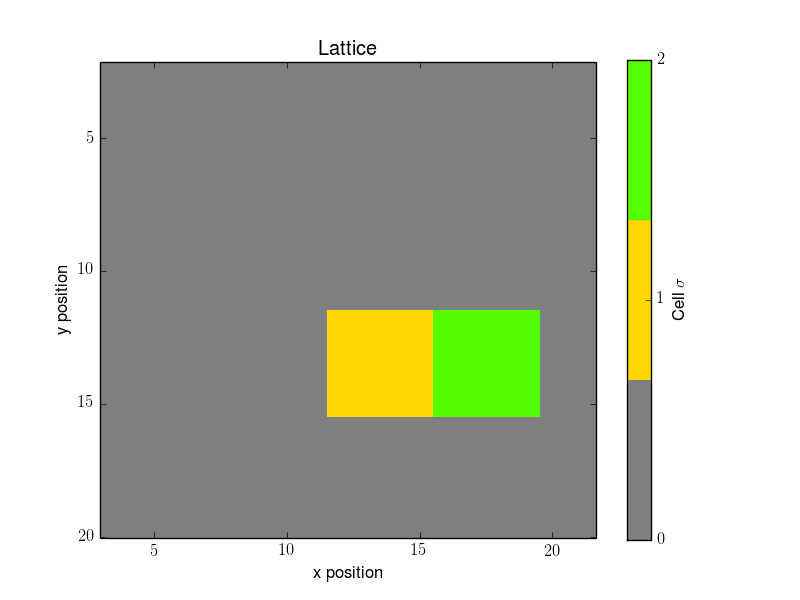
\includegraphics[scale=0.5]{img/basic}
	\caption{An example of two cells in a lattice, each color represents a different cell $\sigma$. The grey area is the Extra Cellular Matrix}
	\label{basic}
\end{figure}
\begin{figure}[h!]
	\centering
	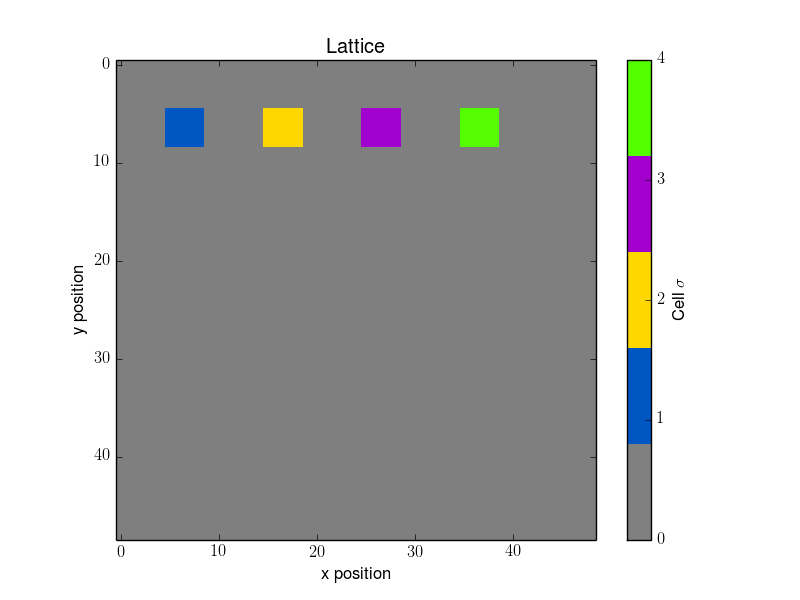
\includegraphics[scale=0.5]{img/before_race_single}
	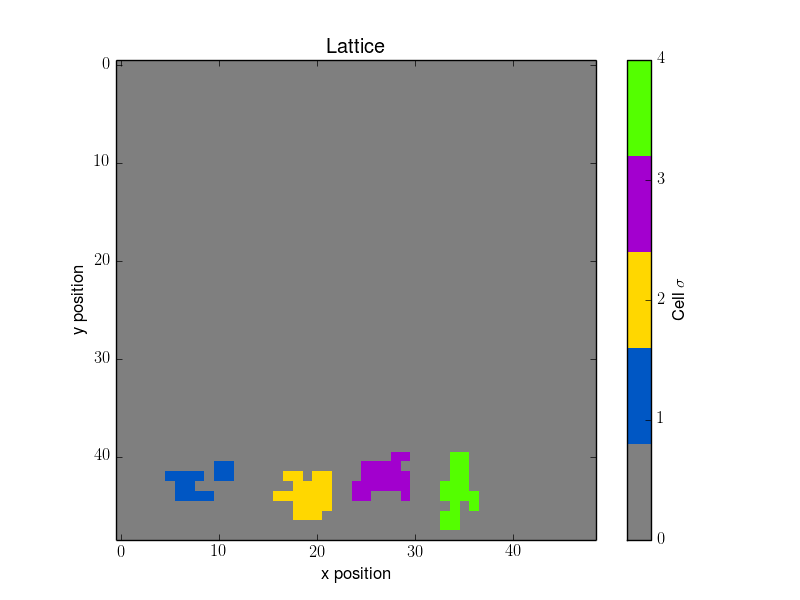
\includegraphics[scale=0.5]{img/after_race_single}
	\caption{A race between four cells: Top image is before the race was conducted and bottom image shows the typical positions of the cells after the race concludes ($8000MCS$)}
	\label{single_race}
\end{figure}
\pagebreak

\bibliographystyle{abbrv}
\bibliography{396}

\section{Appendix: Experimental Conditions}
\begin{enumerate}
	\item Race between single cells was conducted 44 times. Energies were typical to detailed in Materials and Methods. We added Y-potential $F(y)=52y$
\end{enumerate}

\end{document}